\section{Introduction}\label{introduction}

The activity and function of a protein is tightly regulated by its
cellular environment. To interact with their surroundings, proteins use
various types of binding modules that each display distinct binding
properties (\cite{10550212}). One prominent type of binding module
consists of short linear motifs (SLiMs) (\cite{18508681}). These compact
binding sites are generally located in intrinsically disordered regions
(IDR) of the proteome and commonly bind to structured domains in their
interaction partners (\cite{21909575}). SLiMs mediate different types of
interactions that regulate protein functionality, and hence are
important regulators of the dynamic processes involved in cell
signalling (\cite{22480932}) (\cite{24926813}) (Figure 1). The number of
SLiM instances in the human proteome is currently suggested to be over
one million (\cite{25038412}). Identifying SLiMs and elucidating their
functionality is an essential step in understanding cell regulation. The
Eukaryotic Linear Motif (ELM) resource contributes to this process by
providing the necessary tools to researchers working on motifs. It
consists of a database and a prediction tool. The database provides a
categorised repository of experimentally validated linear motif classes
and instances that were manually annotated form the literature. The ELM
prediction tool in turn relies on annotated data, both from the ELM
database and other resources, to accurately analyse unknown sequences
for candidate motifs and assist researchers in selecting the most
plausible ones for experimental validation and discard likely false
positive hits, saving them valuable time and assets (\cite{22110040}).
The following protocols will guide users through the different ELM
applications, explaining how to browse the curated data available in
ELM, how to analyse a protein sequence for putative motifs, and how to
interpret these data and avoid common pitfalls in SLiM discovery.

\begin{figure}[h!]
\centering
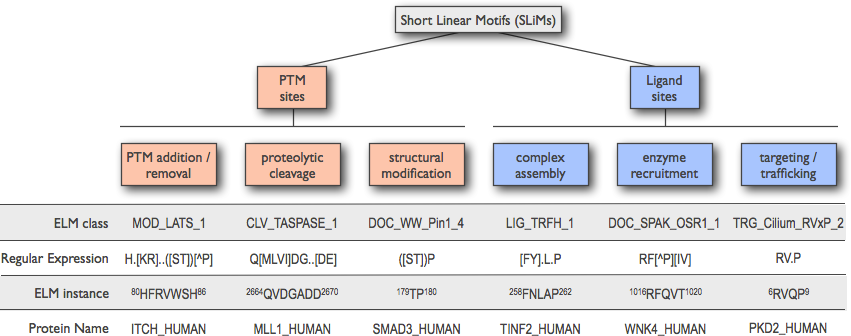
\includegraphics[width=\textwidth]{Figures/functional_classification_of_SLiMs.png}
\caption{
\textbf{Figure functional\_classification\_of\_SLiMs}
For each ELM
class, the functional category to which it belongs is indicated by a
three-letter prefix. Each ELM class is defined by a regular expression.
Peptide sequences in proteins that match the regular expression of a
specific ELM class and that were experimentally validated to be
functional motifs are captured as ELM instances of that class. Degrons
are a specific subtype of enzyme-recruiting docking motifs (see text for
a detailed description).
}
\end{figure}
